\section{Complete Abrial Example}
\label{tutorial_10}

\tick{\textbf{Goals:} The objective of this section is to create a model of the Location Access Controler, and besides detail more complex proofs in order to approach the notion of deadlock freeness.
}
\info {First of all you need to download the following file named doors.zip}
\subsection{Project Setup}
Import the archive file doors.zip, for this select  \textsf{File $\rangle$ Import $\rangle$ General $\rangle$ Existing Project into workspace}, and find your file.
\begin{center}
	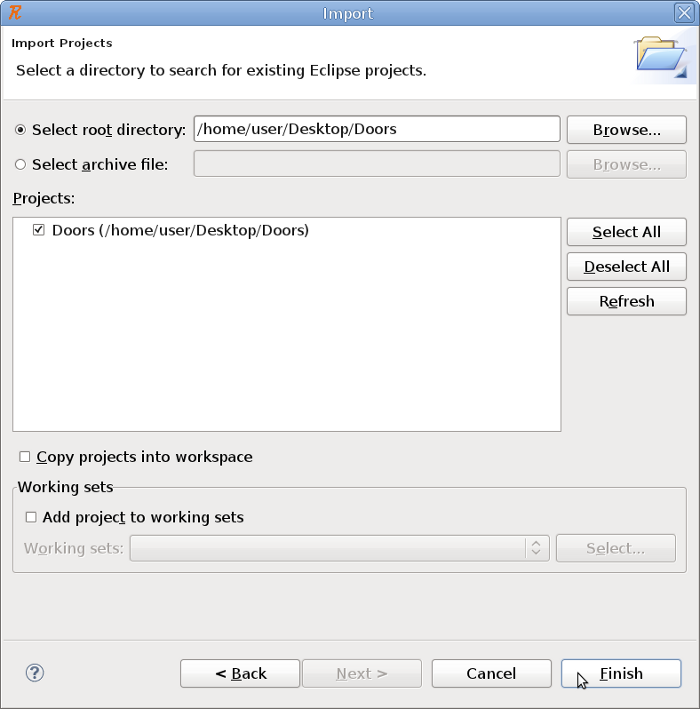
\includegraphics[]{img/tutorial/import.png}
\end{center}
The tool takes a few seconds to extract and load all the files. Once it is done, you can look at the initial model through doors\_ctx1 and doors\_0.
We can notice that there are two carrier sets in the program, actually we have one for the persons and one for locations. Moreover the relation \textbf{aut} represents where people are allowed to go (for example, \textbf{outside} is a location, and everyone is allowed to go \textbf{outside}).

The only \textsf{EVENT} of that model has to aim to change the location of a person.
So, proof of deadlock freeness means proving, that someone can always change room.

Nevertheless you need to add a new derived invariant to doors\_0. We call this invariant \texttt{DLF}.
In the same time, add the associated predicate which is the disfunction of all guards: there is only one guard here, so it would be,
\[
\exists p,l.(p \longmapsto l \in aut \land sit(p) \neq l )
\]


\begin{center}
	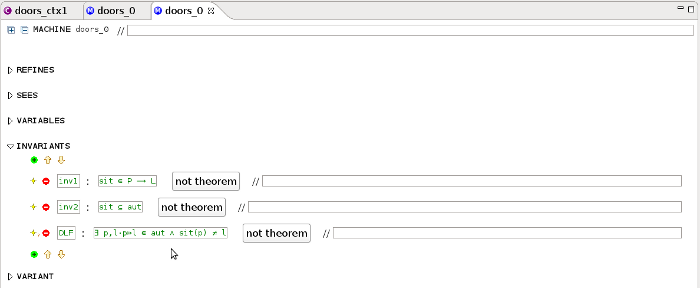
\includegraphics[]{img/tutorial/new-invariant.png}
\end{center}

\subsubsection{Autoprover}

Save the machine.



\textbf{here your in text bold}
